%
%  2-intelligent-agents.tex
%  Introduction To Artificial Intelligence
%
%  Created by Illya Starikov on 01/23/18.
%  Copyright 2018. Illya Starikov. All rights reserved.
%

\section{Intelligent Agents}
\begin{itemize}
    \item Computer agents\ldots
        \begin{itemize}
            \item Perceive environment
            \item Operate autonomously
            \item Persist over prolonged periods
        \end{itemize}

    \item Rational Agents\ldots
        \begin{itemize}
            \item Are affected by their environment.
            \item Use sensors to interpret their environment
            \item From said sensors, it acts on them via actuators
            \item These are summarized by Figure~\ref{fig:diagram}. The main focus of the semester is filling in the \shellcmd{?}.
        \end{itemize}
\end{itemize}

\begin{figure}[htpb]
    \centering
    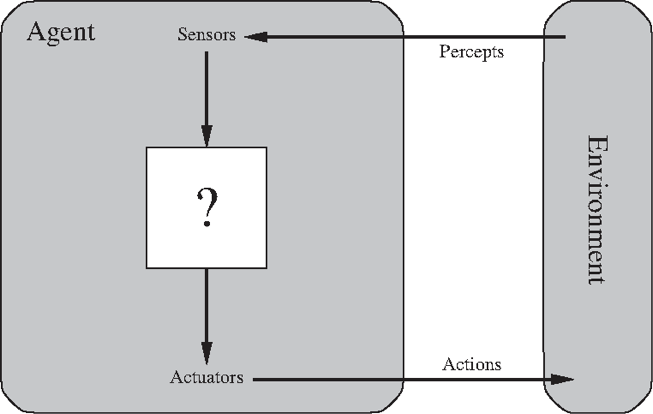
\includegraphics[width=.5\linewidth]{./assets/agent-diagram.png}
    \caption{An Agent Cycle}\label{fig:diagram}
\end{figure}

\begin{itemize}
    \item Rational behavior depends on\ldots
        \begin{itemize}
            \item Agent’s performance measure
            \item Agent’s prior knowledge
            \item Possible percepts and actions
            \item Agent’s percept sequence
        \end{itemize}

    \item We define a rational agents as follows:
        \begin{quote}
            ``For each possible percept sequence, a rational agent selects an action that is expected to maximize its performance measure, given the evidence provided by the percept sequence and any prior knowledge the agent has.''
        \end{quote}

    \item PEAS\footnote{Performance Measure, Environment, Actuators, and Sensors} descriptoin and properties\ldots
        \begin{description}
            \item[Observable/Partially Observable] If it is possible to determine the complete state of the environment at each time point from the percepts it is observable; otherwise it is only partially observable.
            \item[Deterministic/Stochastic/Strategic] If the next state of the environment is completely determined by the current state and the action executed by the agent, then it is determinstic. If the environment is deterministic except for the actions of other agents, then the environment is strategic. If it is randomly determined, then it is stochastic.
            \item[Episodic, Sequential] In an episodic environment, each episode consists of the agent perceiving and then acting. The quality of its action depends just on the episode itself. Subsequent episodes do not depend on the actions in the previous episodes. Episodic environments are much simpler because the agent does not need to think ahead.
            \item[Static/Semi-Dynamic/Dynamic] If an environement is unchanged while an agent is deliberating, it is static. The environment is semi-dynamic if the environment itself does not change with the passage of time but the agent’s performance score does. If the environment is constantly changing, then it is dynamic.
            \item[Discrete/Continuous] If there are a limited number of distinct, clearly defined, states of the environment, the environment is discrete (For example, chess); otherwise it is continuous (For example, driving).
            \item[Discrete/Continuous] If there are a limited number of distinct, clearly defined, states of the environment, the environment is discrete (For example, chess); otherwise it is continuous (For example, driving).
            \item[Single Agent/Multi-Agent] The environment may contain other agents which may be of the same or different kind as that of the agent.
            \item[Competitive/Cooperative] If agents are in direct competition with each other (i.e., chess), they are competitive. If they have a common goal, they are cooperative.
            \item[Known/Unknown] An environment is considered to be known if the agent understands the laws that govern the environment's behavior. For example, in chess, the agent would know that when a piece is ``taken'' it is removed from the game.
        \end{description}

        \item Some agent types include\ldots
            \begin{description}
                \item[Simple Reflex Agents] Simple reflex agents act only on the basis of the current percept, ignoring the rest of the percept history. The agent function is based on the condition-action rule: \shellcmd{if condition then} action.
                \item[Model-Based Reflex Agents] A model-based agent can handle partially observable environments. Its current state is stored inside the agent maintaining some kind of structure which describes the part of the world which cannot be seen. This knowledge about ``how the world works'' is called a model of the world, hence the name ``model-based agent''.
                \item[Goal-Based Agents] Goal-based agents further expand on the capabilities of the model-based agents, by using ``goal'' information. Goal information describes situations that are desirable. This allows the agent a way to choose among multiple possibilities, selecting the one which reaches a goal state. Search and planning are the subfields of artificial intelligence devoted to finding action sequences that achieve the agent's goals.
                \item[Utility-Based Agents] Goal-based agents only distinguish between goal states and non-goal states. It is possible to define a measure of how desirable a particular state is. This measure can be obtained through the use of a utility function which maps a state to a measure of the utility of the state. A more general performance measure should allow a comparison of different world states according to exactly how happy they would make the agent. The term utility can be used to describe how ``happy'' the agent is.
                \item[Learning Agents] Learning has the advantage that it allows the agents to initially operate in unknown environments and to become more competent than its initial knowledge alone might allow. The most important distinction is between the ``learning element'', which is responsible for making improvements, and the ``performance element'', which is responsible for selecting external actions.
            \end{description}

            \item The definition of a problem solving agent is as follows\ldots
                \begin{quote}
                    Problem-solving agents are goal based agents that decide what to do based on an action sequence leading to a goal state.
                \end{quote}
\end{itemize}
